\documentclass{elegantbook}
\usepackage[square,numbers,sort&compress]{natbib}
\newcommand{\upcite}[1]{\textsuperscript{\textsuperscript{\cite{#1}}}}
\usepackage{multirow}
\usepackage{tikz}
\usetikzlibrary{shapes.geometric, arrows}
\tikzstyle{startstop} = [rectangle, rounded corners, minimum width = 2cm, minimum height=1cm,text centered, draw = black, fill = red!40]
\tikzstyle{acti} = [trapezium, trapezium left angle=70, trapezium right angle=110, minimum width=2cm, minimum height=1cm, text centered, draw=black, fill = blue!40]
\tikzstyle{process} = [rectangle, minimum width=3cm, minimum height=1cm, text centered, draw=black, fill = green!50]
\tikzstyle{loss} = [rectangle, rounded corners, minimum width = 2cm, minimum height=1cm,text centered, draw = black, fill = yellow!40]
\tikzstyle{arrow} = [->,>=stealth]

% title info
\title{Deep Learning}
\subtitle{MNIST Digits Classification with MLP}
% bio info
\author{Yantian Luo}
\institute{Electronic Engineering}
\version{2018310742}
\date{\today}
\logo{logo.png}
\cover{cover.jpg}

\begin{document}

\maketitle
\tableofcontents
\mainmatter
\hypersetup{pageanchor=true}
% add preface chapter here if needed
\chapter{Introduction}
MNIST digits dataset is a widely used database for image classification in machine learning field. It contains 60,000 training samples and 10,000 testing samples. Each sample is a $784\times1$ column vector, which is transformed from an original $28\times28$ pixels grayscale image.

In this homework, we use multilayer perceptron (MLP) to perform digits classification. We construct a neural network with one hidden layer and two hidden layers to compare the results. We also use Relu and Sigmoid as activation functions to compare different results. And we also compare the differenc ebetween EuclideanLoss and SoftmaxCrossEntropyLoss for all the above experiments.

\chapter{Algorithm Design}
For multilayer perceptron, forward and backward is most important. Forward represents the data processing performed by the layer and backward performs backpropagation operations. According to the chain rule, the most import thing for backward is compute the derivation of output with respect to input. In this chapter, we compute and derive the data processing formula of forward and backward.

\section{Layers}
In this section, we compute and derive the formula of three types of layers, which are Relu, Sigmoid and Linear layers.

\subsection{Relu layer}
Figure \ref{relu} show the Relu functions. 
\begin{figure}[!ht]
	\centering
	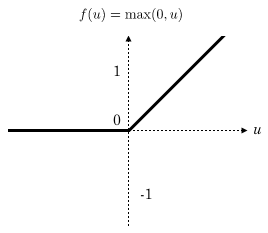
\includegraphics[width=0.6\textwidth]{relu1.png}
	\caption{\label{relu}Relu activation functions}
\end{figure}

Suppose the input of Relu layer is $X$, and the output is $Y$. According to relu function, we can get forward operation as formula (\ref{relueq}).
\begin{equation}\label{relueq}\begin{aligned}
Y&=\left\{\begin{array}{cc}
X & X>0 \\
0 & X\le 0
\end{array}\right. \\
&=\max\{0,X\}
\end{aligned}
\end{equation}
And we can easily get the derivation of it as follow:
\begin{equation}
\label{brelu}
\frac{\partial Y}{\partial X}=\left\{\begin{array}{cc}
1 & X>0 \\
0 & X\le 0
\end{array}\right.
\end{equation}

\subsection{Sigmoid layer}
Figure \ref{sigmoid} show the Sigmoid functions. 
\begin{figure}[!ht]
	\centering
	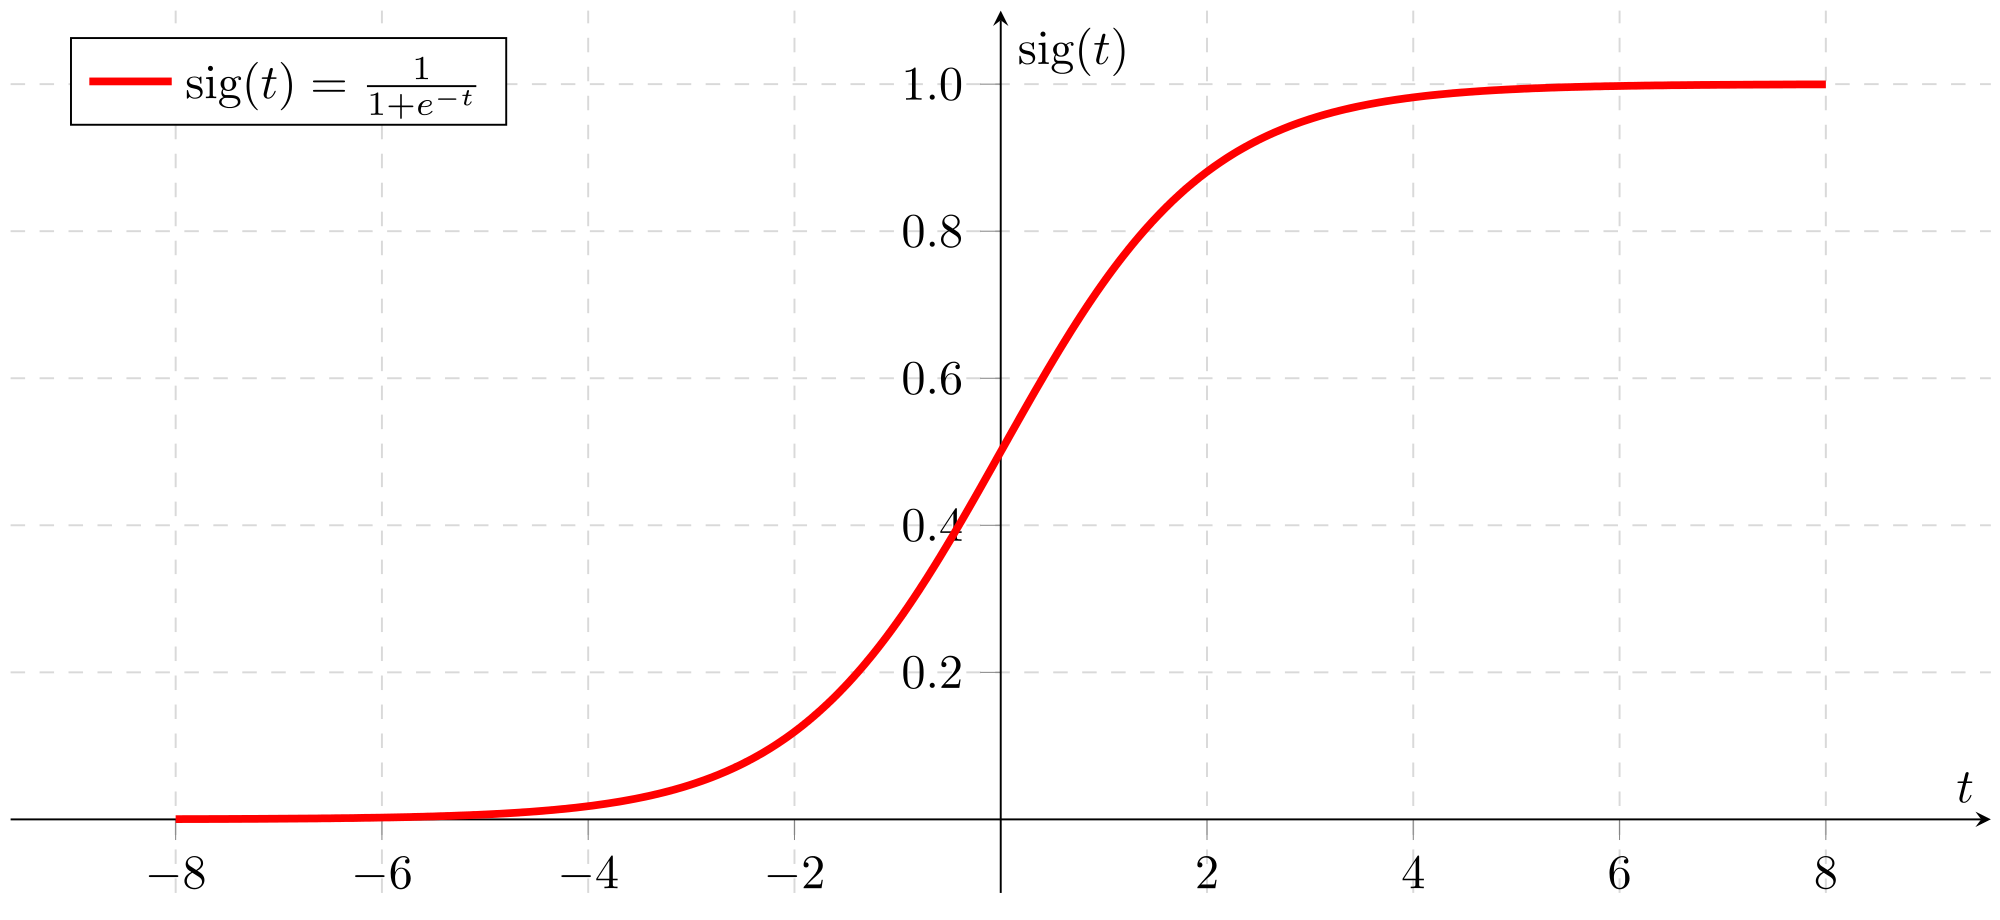
\includegraphics[width=0.8\textwidth]{Sigmoid.png}
	\caption{\label{sigmoid}Sigmoid activation functions}
\end{figure}

Suppose the input of Relu layer is $X$, and the output is $Y$. According to sigmoid function, we can get forward operation as formula (\ref{sigmoideq}).
\begin{equation}
\label{sigmoideq}
Y = \frac{1}{1+e^{-X}}
\end{equation}
Then we can compute the derivation of $Y$ with respect to $X$ as follow:
\begin{equation}
\begin{aligned}
\frac{\partial Y}{\partial X}&=\dfrac{e^{-x}}{\left(1+e^{-x}\right)^2} \\
&=\frac{1}{1+e^{-x}}\cdot\frac{e^{-x}}{1+e^{-x}} \\
&=Y(1-Y)
\end{aligned}
\end{equation}

\subsection{Linear layer}
Figure \ref{linear} show the linear layer. 
\begin{figure}[!ht]
	\centering
	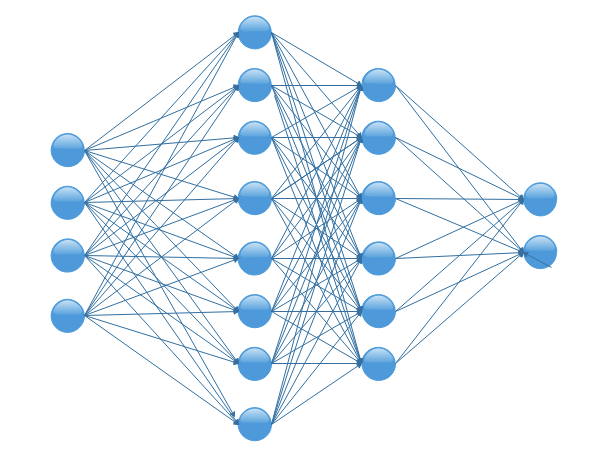
\includegraphics[width=0.6\textwidth]{linear.png}
	\caption{\label{linear}Linear layer (also called fully connected layer)}
\end{figure}

Suppose the input of linear layer is $X$, and the output is $Y$. Assuming the weight matrix is $W$ and the bias vector is $b$, then we have formula (\ref{sigmoideq}).
\begin{equation}
\label{lineareq}
Y = W\cdot X + b
\end{equation}
Then we can compute the derivation of $Y$ with respect to $X, W, b$ as follow:
\begin{equation}
\left\{
\begin{aligned}
\frac{\partial Y}{\partial X}&=W \\
\frac{\partial Y}{\partial W}&=X \\
\frac{\partial Y}{\partial b}&=1
\end{aligned}\right.
\end{equation}

\section{Losses}
In this section, we compute the forward and backward formulas of two types of losses: EuclideanLoss and SoftmaxCrossEntropyLoss.

\subsection{EuclideanLoss}
Suppose the predict label is $y$ and the true label is $T$. And assuming the $T$ is in one-hot encoding form.

\subsubsection{Forward}
Assuming the batchsize is $N$, we can derivate the EuclideanLoss as follow:
\begin{equation}
E=\frac{1}{2N}\sum_{n=1}^{N}\left||T(n)-y(n)|\right|^2
\end{equation}
\subsubsection{Backward}
We can compute the derivation of $E$ with respect to $y$ as follow:
\begin{equation}
\begin{aligned}
\frac{\partial E}{\partial y(n)}=&\frac{1}{2N}\cdot 2(y(n)-T(n)) \\
=&\frac{1}{N}\left[y(n)-T(n)\right] \\
&\forall n=1,2,\cdots,N
\end{aligned}
\end{equation}

\subsection{SoftmaxCrossEntropyLoss}
Suppose the predict label is $x$ and the true label is $t$. And assuming the $t$ is in one-hot encoding form. 

\subsubsection{Forward}
To compute the SoftmaxCrossEntropyLoss, we need three steps:
\begin{itemize}
	\item Compute softmax of each label;
	\begin{equation}
	h_k^{(n)}=P(t_k^{(n)}=1|x^{(n)})=\dfrac{\exp(x_k^{(n)})}{\sum_{j=1}^{K}\exp(x_j^{(n)})}
	\end{equation}
	\item Compute crossentropy;
	\begin{equation}
	E^{(n)}=-\sum_{k=1}^{K}t_k^{(n)}\ln h_k^{(n)}
	\end{equation}
	\item Compute Loss;
	\begin{equation}
	E=\frac{1}{N}\sum_{n=1}^{N}E^{(n)}
	\end{equation}
\end{itemize}

\subsection{Backward}
We use the chain rule to compute the derivation of $E$ with respect to $x$ as follow:
\begin{equation}
\frac{\partial E}{\partial x^{(n)}}=\frac{\partial E}{\partial E^{(n)}}\frac{\partial E^{(n)}}{\partial x^{(n)}}
\end{equation}

First, we compute $\frac{\partial E^{(n)}}{\partial x^{(n)}}$ as follow:
\begin{equation}
\begin{aligned}
\frac{\partial E^{(n)}}{\partial x_k^{(n)}}&=\sum_{i=1}^K\frac{\partial E^{(n)}}{\partial h_i^{(n)}}\frac{\partial h_i^{(n)}}{\partial x_k^{(n)}} \\
&=\sum_{i=1}^K\left(-t_i^{(n)}\frac{1}{h_i^{(n)}}\right)\frac{\partial h_i^{(n)}}{\partial x_k^{(n)}}
\end{aligned}
\end{equation}

Then we compute $\frac{\partial h_i^{(n)}}{\partial x_k^{(n)}}$ to get $\frac{\partial E^{(n)}}{\partial x^{(n)}}$:
\begin{equation}
\begin{aligned}
\frac{\partial h_i^{(n)}}{\partial x_k^{(n)}}&=\left\{
\begin{array}{cc}
h_i^{(n)}(1-h_k^{(n)})& i=k \\
-h_i^{(n)}h_k^{(n)} & i\ne k
\end{array}
\right. \\
&=h_i^{(n)}(\bigtriangleup_{i,k}-h_k^{(n)}) \\
&where\quad \bigtriangleup_{i,k}=\left\{
\begin{array}{cc}
1 & i=k \\
0 & i\ne k
\end{array}
\right.
\end{aligned}
\end{equation}

Then we have:
\begin{equation}
\begin{aligned}
\frac{\partial E^{(n)}}{\partial x_k^{(n)}}&=\sum_{i=1}^K\left(-t_i^{(n)}\frac{1}{h_i^{(n)}}\right)h_i^{(n)}(\bigtriangleup_{i,k}-h_k^{(n)}) \\
&=\sum_{i=1}^K\left(-t_i^{(n)}\bigtriangleup_{i,k}\right)+\sum_{i=1}^Kt_i^{(n)}h_k^{(n)} \\
&=-(t_k^{(n)}-h_k^{(n)})
\end{aligned}
\end{equation}

Therefore, we can compute the backward formula:
\begin{equation}
\begin{aligned}
\frac{\partial E}{\partial x_k^{(n)}}&=\frac{\partial E}{\partial E^{(n)}}\frac{\partial E^{(n)}}{\partial x^{(n)}} \\
&=-\frac{1}{N}(t_k^{(n)}-h_k^{(n)})
\end{aligned}
\end{equation}

\chapter{Experients and Results}

In this chapter, we compare the difference of Relu vs. Sigmoid active functions, EuclideanLoss vs. SoftmaxCrossEntropyLoss in one hidden layer network and two hidden layers network.

\section{One hidden layer experiments}
The network structure in this section is designed as Figure \ref{fig1} and training arguments is as follow:

\begin{lstlisting}[frame=single,language=python]  
config = {
	'learning_rate': 0.1,
	'weight_decay': 0.0001,
	'momentum': 0.001,
	'batch_size': 100,
	'max_epoch': 100,
	'disp_freq': 50,
}
\end{lstlisting}

\begin{figure}[htbp]
	\centering
	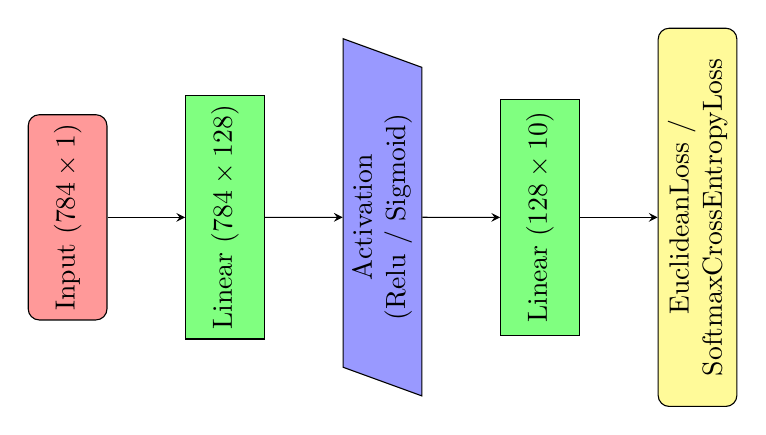
\begin{tikzpicture}
		\node (start) [startstop, rotate=90] {Input ($784\times 1$)};
		\node (linear1) [process, rotate=90, below of=start, yshift=-1cm] {Linear ($784\times 128$)};
		\node (acti1) [acti, rotate=90, below of=linear1, yshift=-1cm, text width=10em] {Activation \\(Relu / Sigmoid)};
		\node (linear2) [process, rotate=90, below of=acti1, yshift=-1cm] {Linear ($128\times 10$)};
		\node (loss) [loss, rotate=90, below of=linear2, yshift=-1cm, text width=13em] {EuclideanLoss /\\ SoftmaxCrossEntropyLoss};
		
		\draw [arrow](start) -- (linear1);
		\draw [arrow](linear1) -- (acti1);
		\draw [arrow](acti1) -- (linear2);
		\draw [arrow](linear2) -- (loss);
	\end{tikzpicture}
	\caption{\label{fig1}Network Structure with one hidden layer}
\end{figure}

%\begin{table}[!ht]
%	\centering
%	\caption{\label{tab1}Network Structure with one hidden layer}
%	\begin{tabular}{|c|c|c|c|c|c|}
%		\hline
%		layer name & Input & Linear & Activation & Linear & Loss \\
%		\hline
%		\multirow{2}{*}{Size} & \multirow{2}{*}{$784 \times 1$} & \multirow{2}{*}{$784 \times 128$} & Relu & \multirow{2}{*}{$128\times 10$} &  EuclideanLoss \\
%		 & & & Sigmoid & &SoftmaxCrossEntropyLoss \\
%		\hline
%	\end{tabular}
%\end{table}

\subsection{Using Relu and EuclideanLoss}
First we use Relu as activation function and EuclideanLoss as loss function to take the experiment.


Then we draw the train accuracy curve and train loss curve as shown in \ref{traincurve1} and we draw the test accuracy curve and test loss curve with respect to epoch as shown in \ref{testcurve1}
\begin{figure}[!ht]
	\centering
	\begin{minipage}[t]{0.45\textwidth}
		\centering
		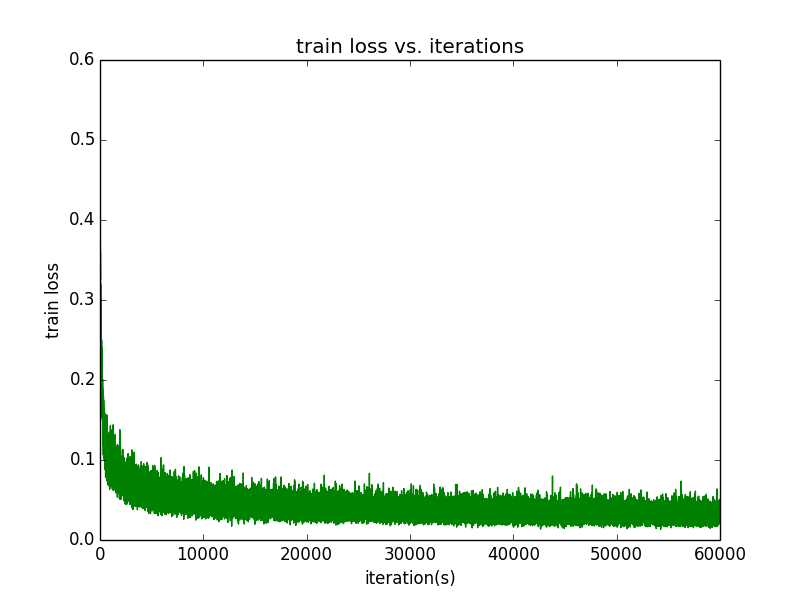
\includegraphics[width=\textwidth]{trainloss1re}
	\end{minipage}
	\begin{minipage}[t]{0.45\textwidth}
		\centering
		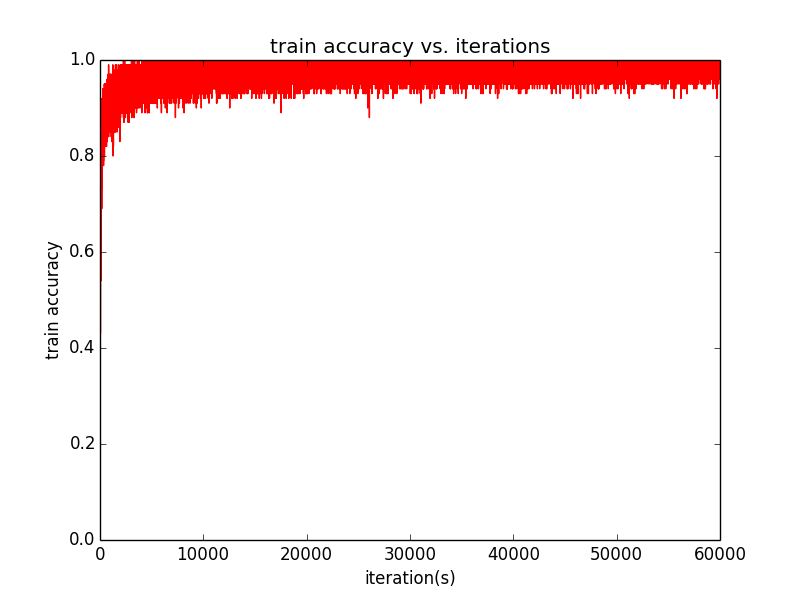
\includegraphics[width=\textwidth]{trainacc1re}
	\end{minipage}
	\caption{\label{traincurve1}train loss curve and train accuracy curve with one hidden layer, Relu activation function and EuclideanLoss}
\end{figure}
\begin{figure}[!ht]
	\centering
	\begin{minipage}[t]{0.45\textwidth}
		\centering
		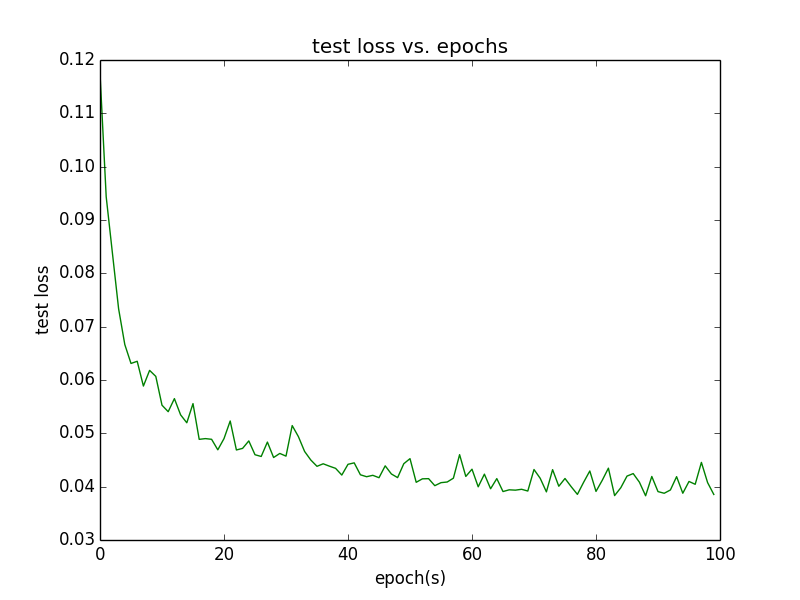
\includegraphics[width=\textwidth]{testloss1re}
	\end{minipage}
	\begin{minipage}[t]{0.45\textwidth}
		\centering
		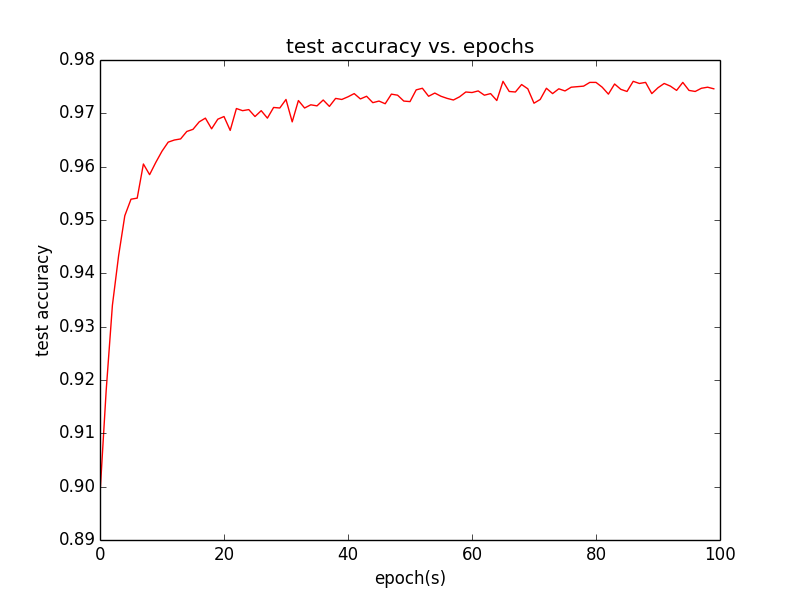
\includegraphics[width=\textwidth]{testacc1re}
	\end{minipage}
	\caption{\label{testcurve1}test loss curve and test accuracy curve with one hidden layer, Relu activation function and EuclideanLoss}
\end{figure}

\subsection{Using Sigmoid and EuclideanLoss}
Then we use Sigmoid as activation function and EuclideanLoss as loss function to take the experiment.


Next we draw the train accuracy curve and train loss curve as shown in \ref{traincurve2} and we draw the test accuracy curve and test loss curve with respect to epoch as shown in \ref{testcurve2}
\begin{figure}[!ht]
	\centering
	\begin{minipage}[t]{0.45\textwidth}
		\centering
		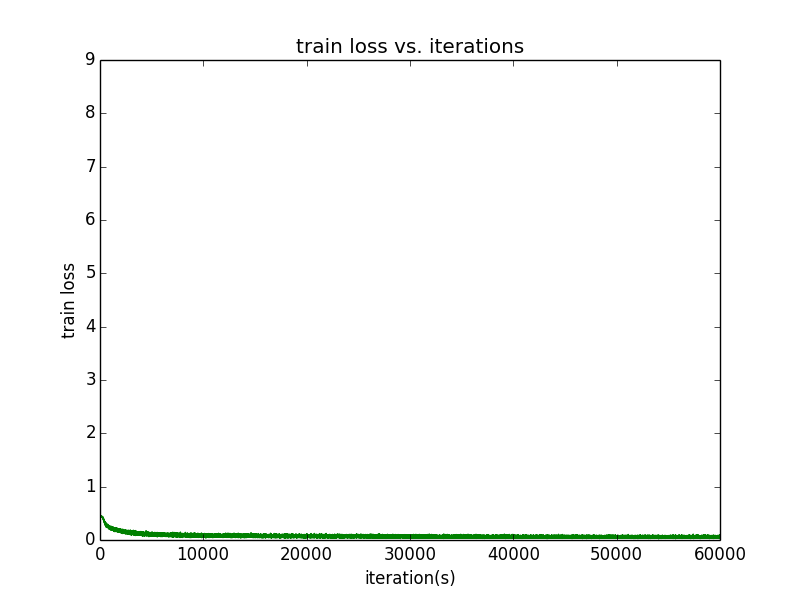
\includegraphics[width=\textwidth]{trainloss1se}
	\end{minipage}
	\begin{minipage}[t]{0.45\textwidth}
		\centering
		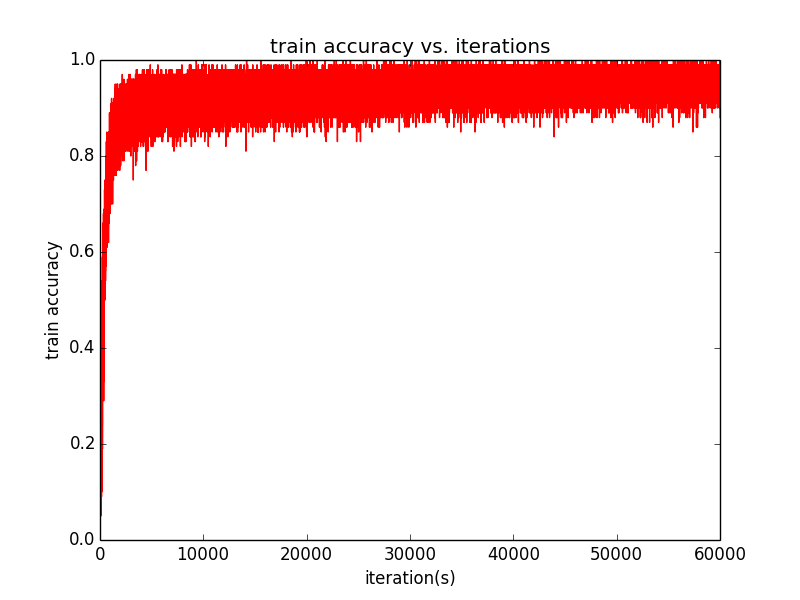
\includegraphics[width=\textwidth]{trainacc1se}
	\end{minipage}
	\caption{\label{traincurve2}train loss curve and train accuracy curve with one hidden layer, Sigmoid activation function and EuclideanLoss}
\end{figure}
\begin{figure}[!ht]
	\centering
	\begin{minipage}[t]{0.45\textwidth}
		\centering
		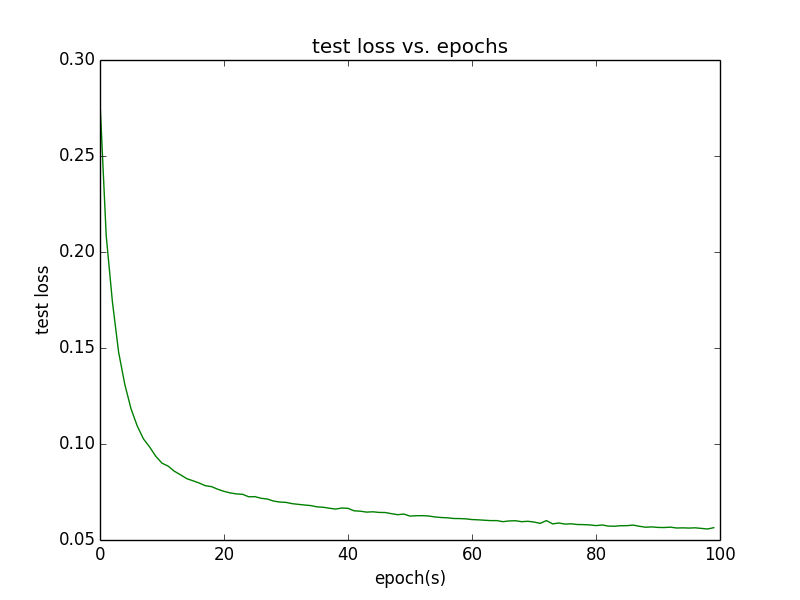
\includegraphics[width=\textwidth]{testloss1se}
	\end{minipage}
	\begin{minipage}[t]{0.45\textwidth}
		\centering
		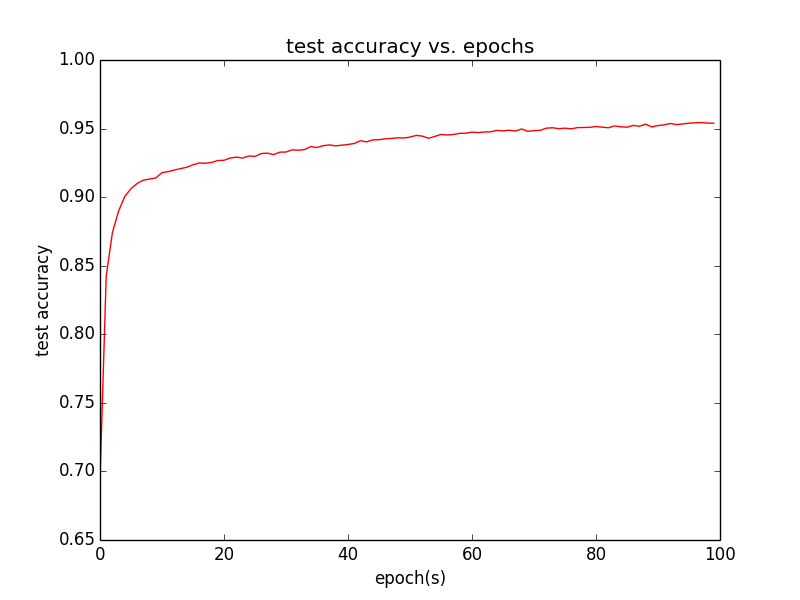
\includegraphics[width=\textwidth]{testacc1se}
	\end{minipage}
	\caption{\label{testcurve2}test loss curve and test accuracy curve with one hidden layer, Sigmoid activation function and EuclideanLoss}
\end{figure}

\subsection{Using Relu and SoftmaxCrossEntropyLoss}
Then we use Relu as activation function and SoftmaxCrossEntropyLoss as loss function to take the experiment.


Next we draw the train accuracy curve and train loss curve as shown in \ref{traincurve3} and we draw the test accuracy curve and test loss curve with respect to epoch as shown in \ref{testcurve3}
\begin{figure}[!ht]
	\centering
	\begin{minipage}[t]{0.45\textwidth}
		\centering
		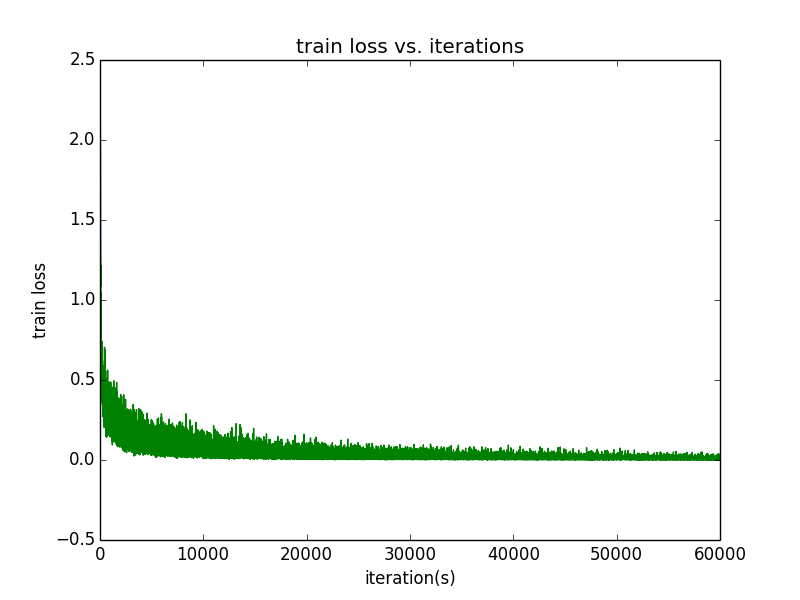
\includegraphics[width=\textwidth]{trainloss1rs}
	\end{minipage}
	\begin{minipage}[t]{0.45\textwidth}
		\centering
		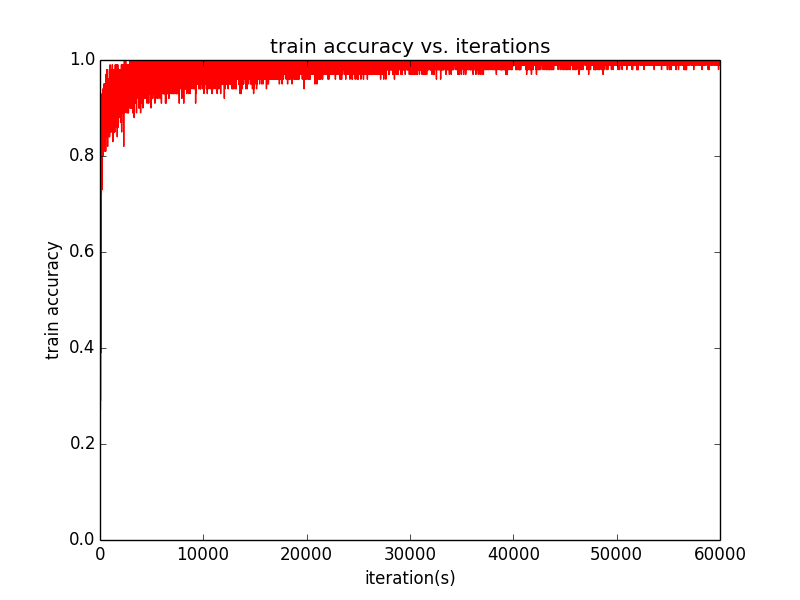
\includegraphics[width=\textwidth]{trainacc1rs}
	\end{minipage}
	\caption{\label{traincurve3}train loss curve and train accuracy curve with one hidden layer, Relu activation function and SoftmaxCrossEntropyLoss}
\end{figure}
\begin{figure}[!ht]
	\centering
	\begin{minipage}[t]{0.45\textwidth}
		\centering
		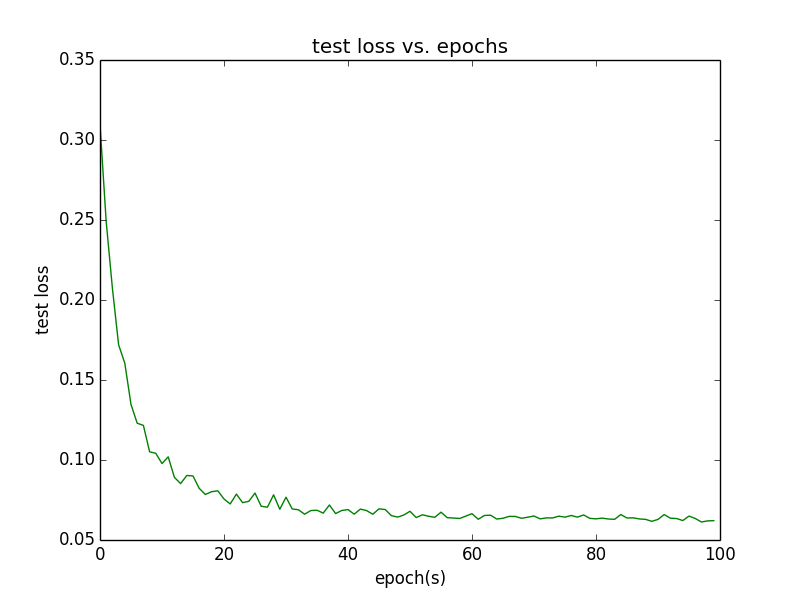
\includegraphics[width=\textwidth]{testloss1rs}
	\end{minipage}
	\begin{minipage}[t]{0.45\textwidth}
		\centering
		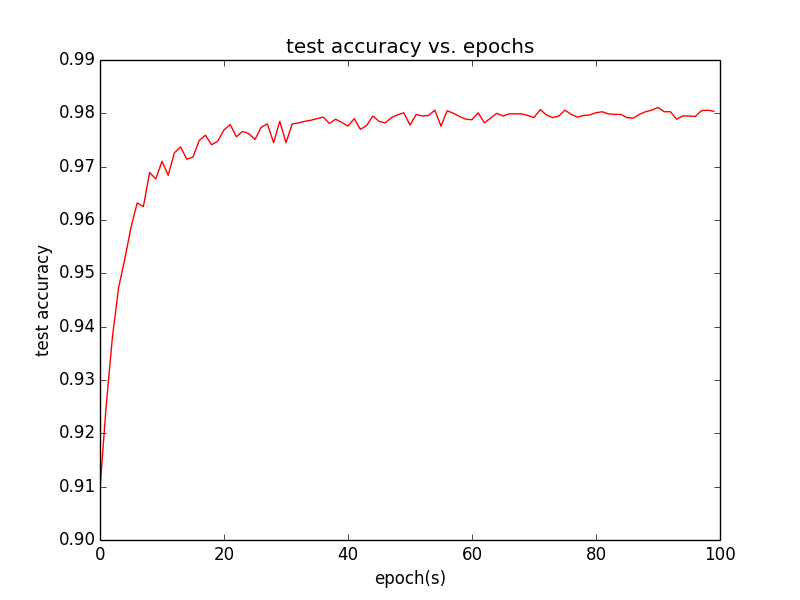
\includegraphics[width=\textwidth]{testacc1rs}
	\end{minipage}
	\caption{\label{testcurve3}test loss curve and test accuracy curve with one hidden layer, Relu activation function and SoftmaxCrossEntropyLoss}
\end{figure}

\subsection{Using Sigmoid and SoftmaxCrossEntropyLoss}
Then we use Sigmoid as activation function and SoftmaxCrossEntropyLoss as loss function to take the experiment.


Next we draw the train accuracy curve and train loss curve as shown in \ref{traincurve3} and we draw the test accuracy curve and test loss curve with respect to epoch as shown in \ref{testcurve3}
\begin{figure}[!ht]
	\centering
	\begin{minipage}[t]{0.45\textwidth}
		\centering
		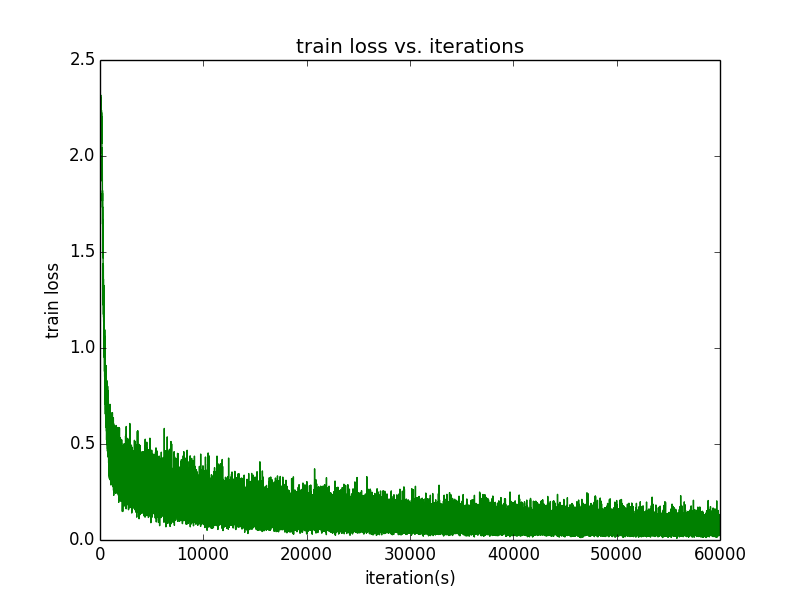
\includegraphics[width=\textwidth]{trainloss1ss}
	\end{minipage}
	\begin{minipage}[t]{0.45\textwidth}
		\centering
		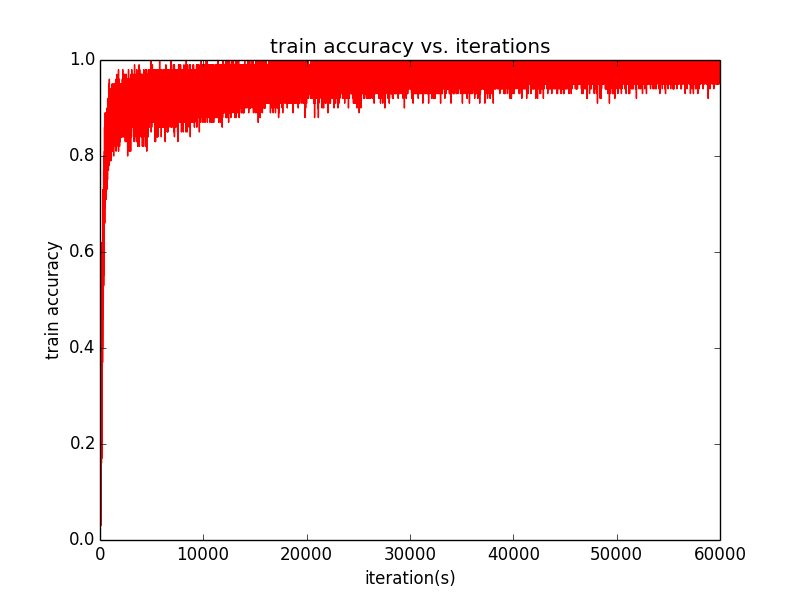
\includegraphics[width=\textwidth]{trainacc1ss}
	\end{minipage}
	\caption{\label{traincurve4}train loss curve and train accuracy curve with one hidden layer, Sigmoid activation function and SoftmaxCrossEntropyLoss}
\end{figure}
\begin{figure}[!ht]
	\centering
	\begin{minipage}[t]{0.45\textwidth}
		\centering
		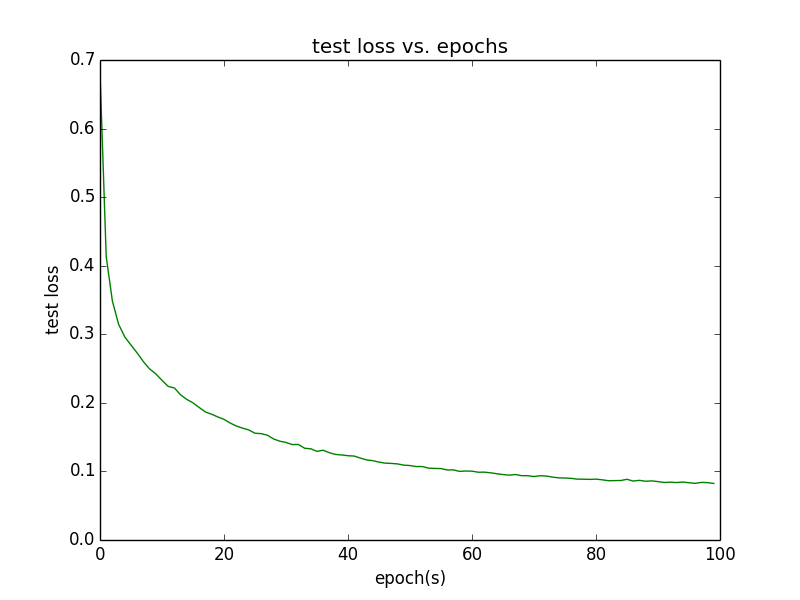
\includegraphics[width=\textwidth]{testloss1ss}
	\end{minipage}
	\begin{minipage}[t]{0.45\textwidth}
		\centering
		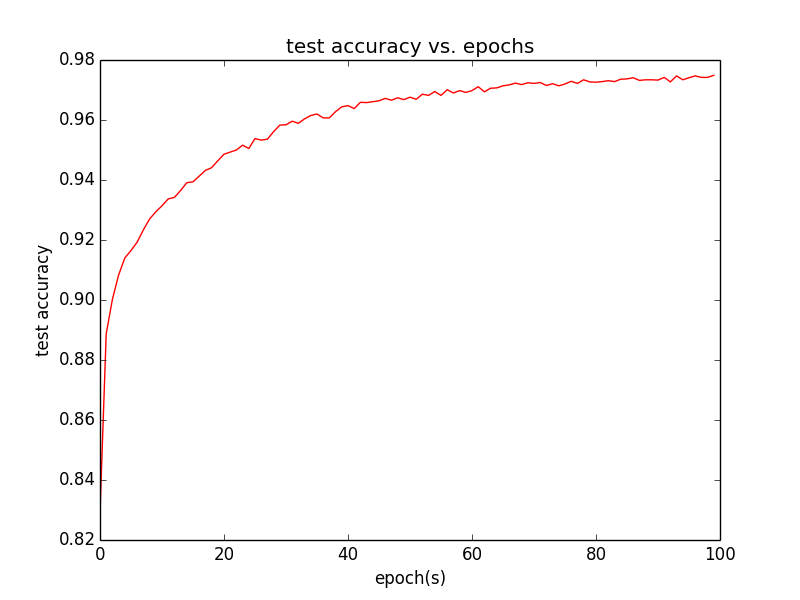
\includegraphics[width=\textwidth]{testacc1ss}
	\end{minipage}
	\caption{\label{testcurve4}test loss curve and test accuracy curve with one hidden layer, Sigmoid activation function and SoftmaxCrossEntropyLoss}
\end{figure}

\section{Two hidden layers experiments}
The network structure in this section is designed as Table\ref{tab2} and training arguments is as follow:

\begin{lstlisting}[frame=single,language=python]  
config = {
    'learning_rate': 0.1,
    'weight_decay': 0.0001,
    'momentum': 0.001,
    'batch_size': 100,
    'max_epoch': 100,
    'disp_freq': 50,
}
\end{lstlisting}

\begin{figure}[htbp]
	\centering
	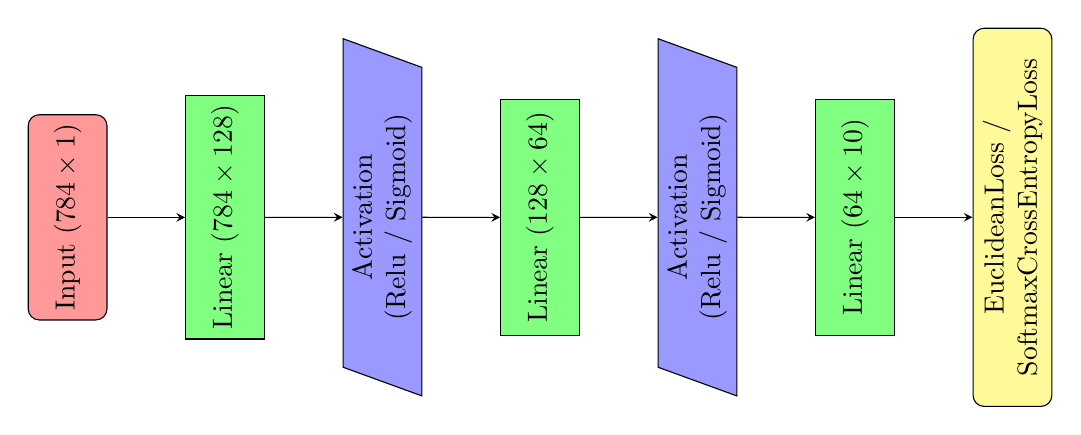
\begin{tikzpicture}
	\node (start) [startstop, rotate=90] {Input ($784\times 1$)};
	\node (linear1) [process, rotate=90, below of=start, yshift=-1cm] {Linear ($784\times 128$)};
	\node (acti1) [acti, rotate=90, below of=linear1, yshift=-1cm, text width=10em] {Activation \\(Relu / Sigmoid)};
	\node (linear2) [process, rotate=90, below of=acti1, yshift=-1cm] {Linear ($128\times 64$)};
	\node (acti2) [acti, rotate=90, below of=linear2, yshift=-1cm, text width=10em] {Activation \\(Relu / Sigmoid)};
	\node (linear3) [process, rotate=90, below of=acti2, yshift=-1cm] {Linear ($64\times 10$)};
	\node (loss) [loss, rotate=90, below of=linear3, yshift=-1cm, text width=13em] {EuclideanLoss /\\ SoftmaxCrossEntropyLoss};
	
	\draw [arrow](start) -- (linear1);
	\draw [arrow](linear1) -- (acti1);
	\draw [arrow](acti1) -- (linear2);
	\draw [arrow](linear2) -- (acti2);
	\draw [arrow](acti2) -- (linear3);
	\draw [arrow](linear3) -- (loss);
	\end{tikzpicture}
	\caption{\label{fig2}Network Structure with two hidden layers}
\end{figure}
%\begin{table}[!ht]
%	\centering
%	\caption{\label{tab2}Network Structure with two hidden layers}
%	\begin{tabular}{|c|c|c|c|}
%		\hline
%		layer name & Input & Linear & Activation  \\
%		\hline
%		\multirow{2}{*}{Size} & \multirow{2}{*}{$784 \times 1$} & \multirow{2}{*}{$784 \times 128$} & Relu \\
%		& & & Sigmoid  \\
%		\hline
%		Linear & Activation & Linear &Loss \\
%		\hline
%		\multirow{2}{*}{$128\times 64$} &  Relu & \multirow{2}{*}{$64\times 10$} &EuclideanLoss \\
%		& Sigmoid & &SoftmaxCrossEntropyLoss \\
%		\hline 
%	\end{tabular}
%\end{table}

\subsection{Using Relu and EuclideanLoss}
First we use Relu as activation function and EuclideanLoss as loss function to take the experiment.


Then we draw the train accuracy curve and train loss curve as shown in \ref{traincurve21} and we draw the test accuracy curve and test loss curve with respect to epoch as shown in \ref{testcurve21}
\begin{figure}[!ht]
	\centering
	\begin{minipage}[t]{0.45\textwidth}
		\centering
		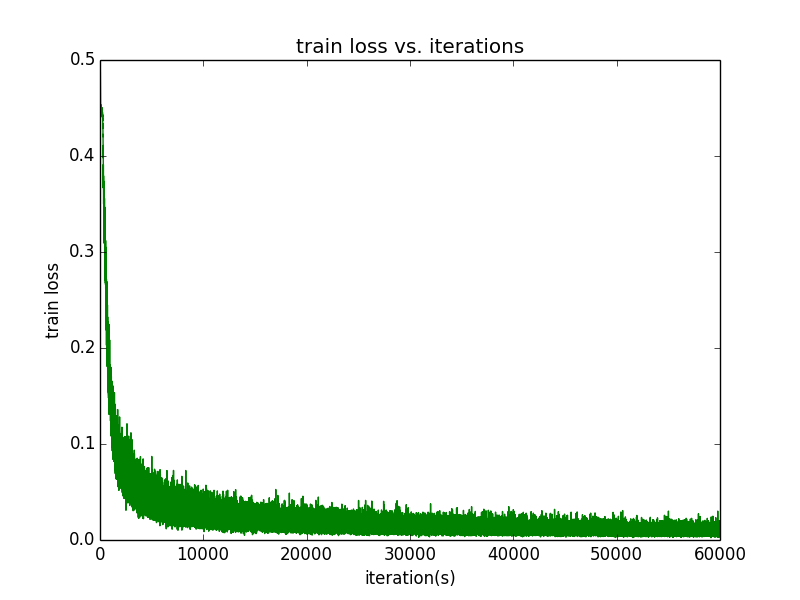
\includegraphics[width=\textwidth]{trainloss2re}
	\end{minipage}
	\begin{minipage}[t]{0.45\textwidth}
		\centering
		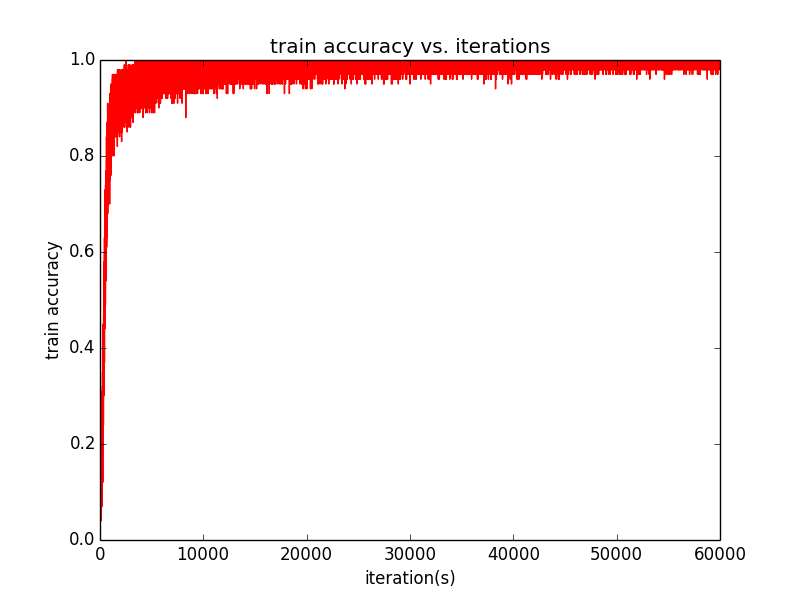
\includegraphics[width=\textwidth]{trainacc2re}
	\end{minipage}
	\caption{\label{traincurve21}train loss curve and train accuracy curve with two hidden layers, Relu activation function and EuclideanLoss}
\end{figure}
\begin{figure}[!ht]
	\centering
	\begin{minipage}[t]{0.45\textwidth}
		\centering
		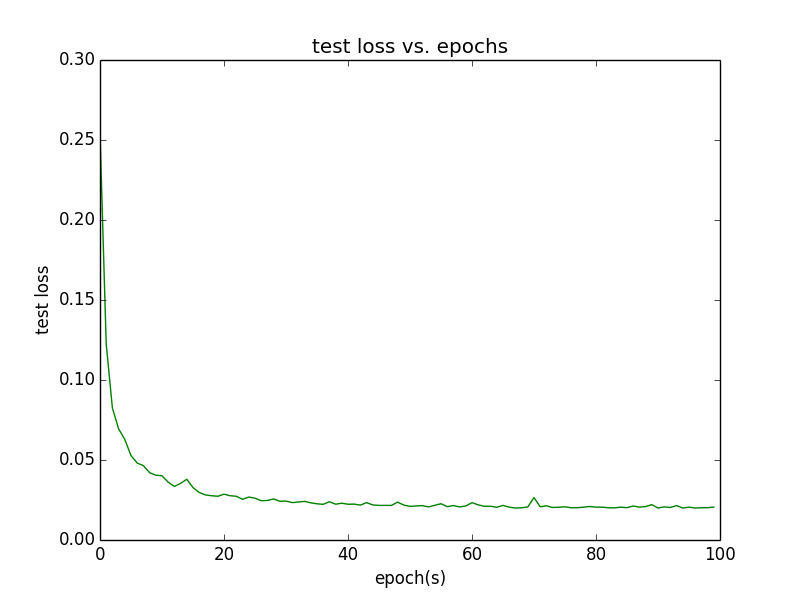
\includegraphics[width=\textwidth]{testloss2re}
	\end{minipage}
	\begin{minipage}[t]{0.45\textwidth}
		\centering
		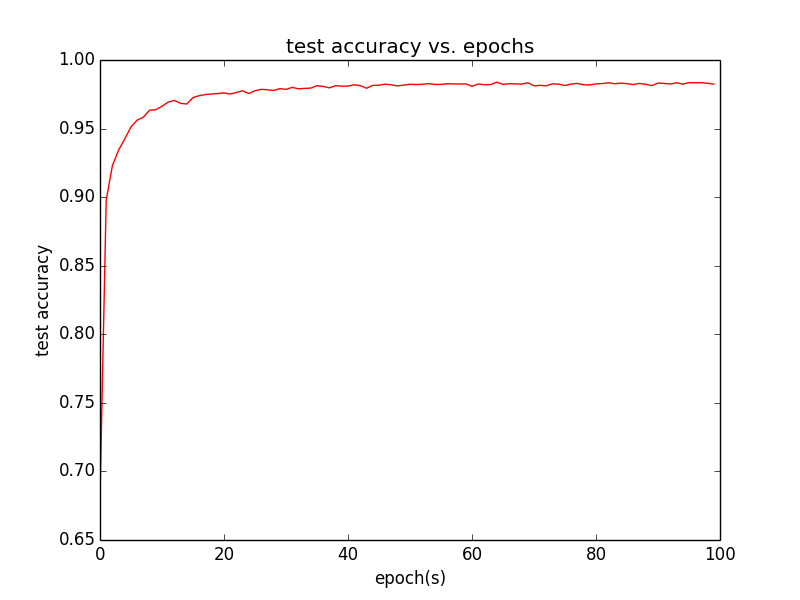
\includegraphics[width=\textwidth]{testacc2re}
	\end{minipage}
	\caption{\label{testcurve21}test loss curve and test accuracy curve with two hidden layers, Relu activation function and EuclideanLoss}
\end{figure}

\subsection{Using Sigmoid and EuclideanLoss}
First we use Sigmoid as activation function and EuclideanLoss as loss function to take the experiment.


Then we draw the train accuracy curve and train loss curve as shown in \ref{traincurve22} and we draw the test accuracy curve and test loss curve with respect to epoch as shown in \ref{testcurve22}
\begin{figure}[!ht]
	\centering
	\begin{minipage}[t]{0.45\textwidth}
		\centering
		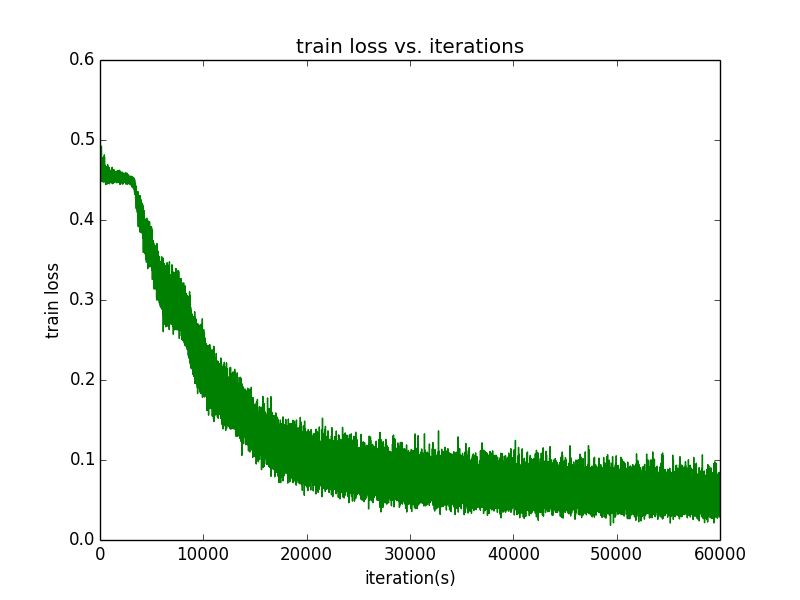
\includegraphics[width=\textwidth]{trainloss2se}
	\end{minipage}
	\begin{minipage}[t]{0.45\textwidth}
		\centering
		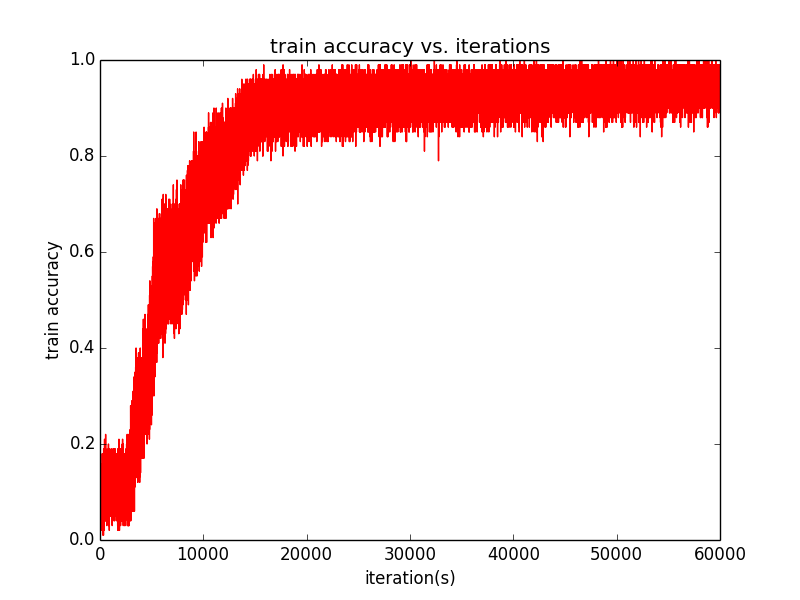
\includegraphics[width=\textwidth]{trainacc2se}
	\end{minipage}
	\caption{\label{traincurve22}train loss curve and train accuracy curve with two hidden layers, Sigmoid activation function and EuclideanLoss}
\end{figure}
\begin{figure}[!ht]
	\centering
	\begin{minipage}[t]{0.45\textwidth}
		\centering
		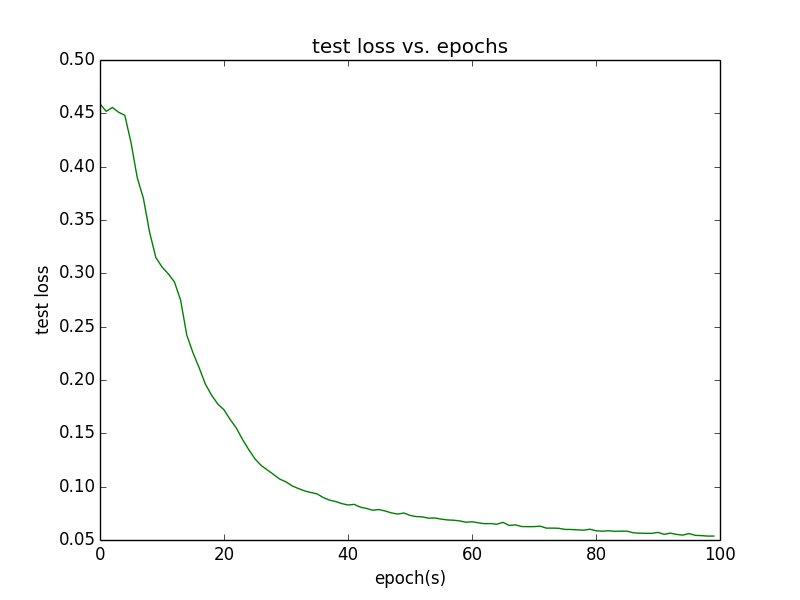
\includegraphics[width=\textwidth]{testloss2se}
	\end{minipage}
	\begin{minipage}[t]{0.45\textwidth}
		\centering
		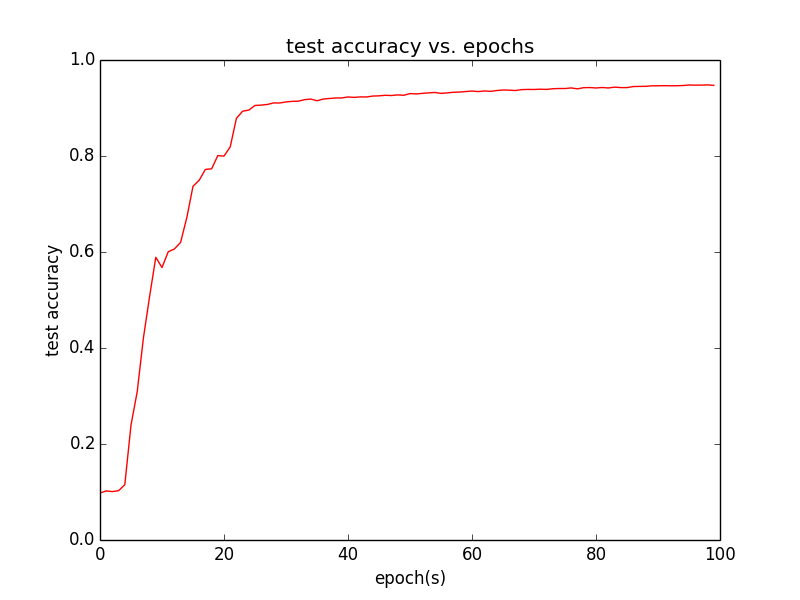
\includegraphics[width=\textwidth]{testacc2se}
	\end{minipage}
	\caption{\label{testcurve22}test loss curve and test accuracy curve with two hidden layers, Sigmoid activation function and EuclideanLoss}
\end{figure}

\subsection{Using Relu and SoftmaxCrossEntropyLoss}
First we use Relu as activation function and SoftmaxCrossEntropyLoss as loss function to take the experiment.


Then we draw the train accuracy curve and train loss curve as shown in \ref{traincurve23} and we draw the test accuracy curve and test loss curve with respect to epoch as shown in \ref{testcurve23}
\begin{figure}[!ht]
	\centering
	\begin{minipage}[t]{0.45\textwidth}
		\centering
		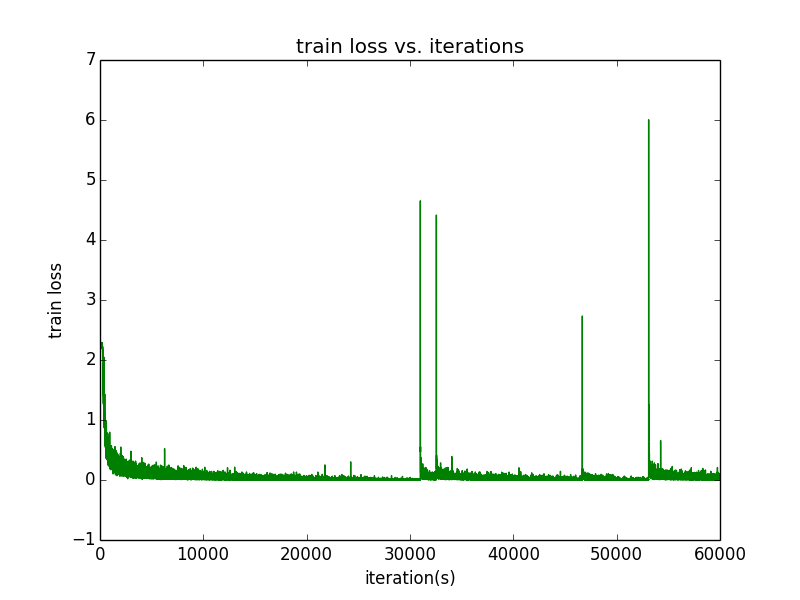
\includegraphics[width=\textwidth]{trainloss2rs}
	\end{minipage}
	\begin{minipage}[t]{0.45\textwidth}
		\centering
		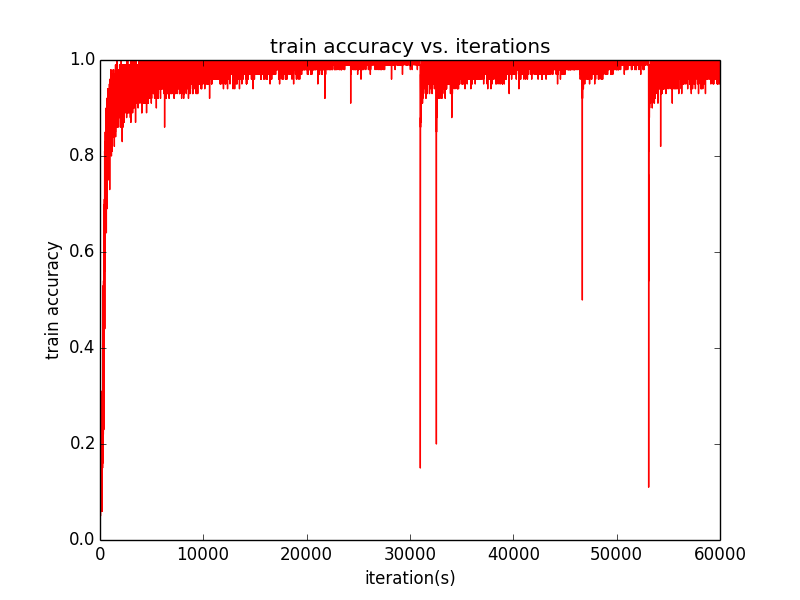
\includegraphics[width=\textwidth]{trainacc2rs}
	\end{minipage}
	\caption{\label{traincurve23}train loss curve and train accuracy curve with two hidden layers, Relu activation function and SoftmaxCrossEntropyLoss}
\end{figure}
\begin{figure}[!ht]
	\centering
	\begin{minipage}[t]{0.45\textwidth}
		\centering
		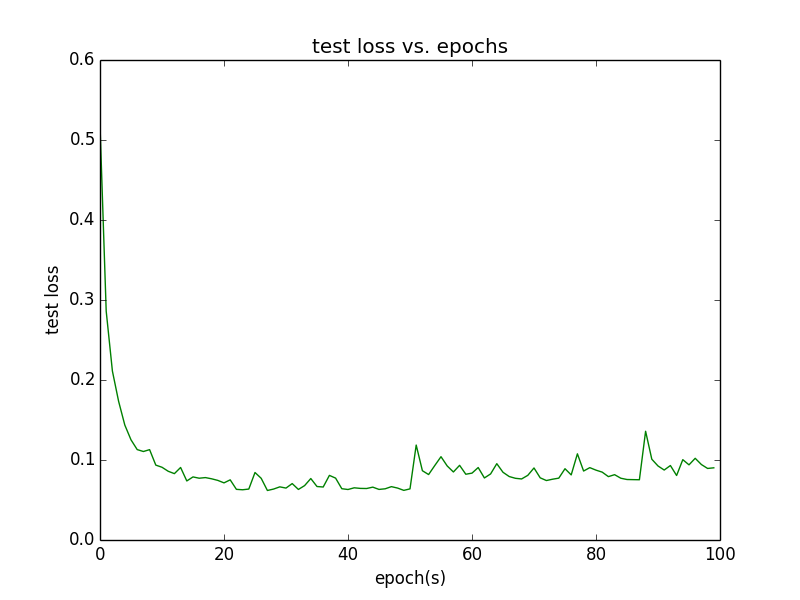
\includegraphics[width=\textwidth]{testloss2rs}
	\end{minipage}
	\begin{minipage}[t]{0.45\textwidth}
		\centering
		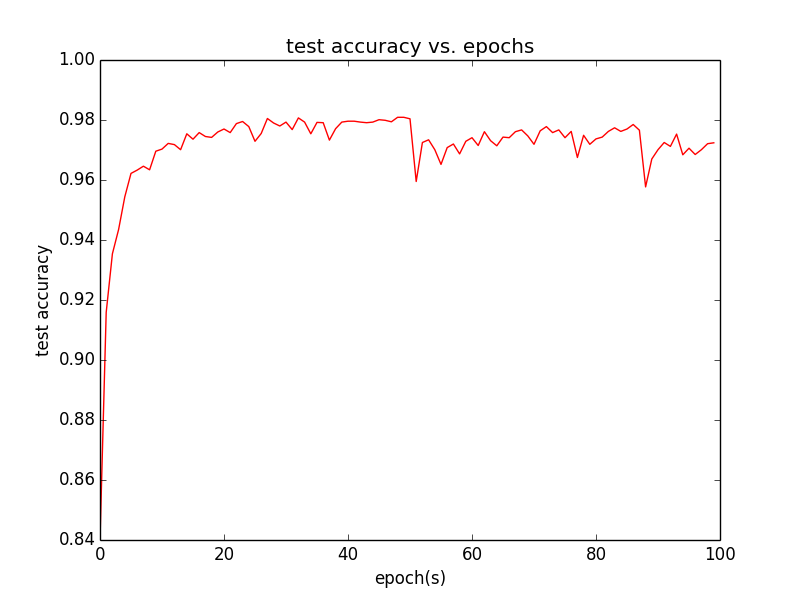
\includegraphics[width=\textwidth]{testacc2rs}
	\end{minipage}
	\caption{\label{testcurve23}test loss curve and test accuracy curve with two hidden layers, Relu activation function and SoftmaxCrossEntropyLoss}
\end{figure}

\subsection{Using Sigmoid and SoftmaxCrossEntropyLoss}
First we use Sigmoid as activation function and SoftmaxCrossEntropyLoss as loss function to take the experiment.


Then we draw the train accuracy curve and train loss curve as shown in \ref{traincurve24} and we draw the test accuracy curve and test loss curve with respect to epoch as shown in \ref{testcurve24}
\begin{figure}[!ht]
	\centering
	\begin{minipage}[t]{0.45\textwidth}
		\centering
		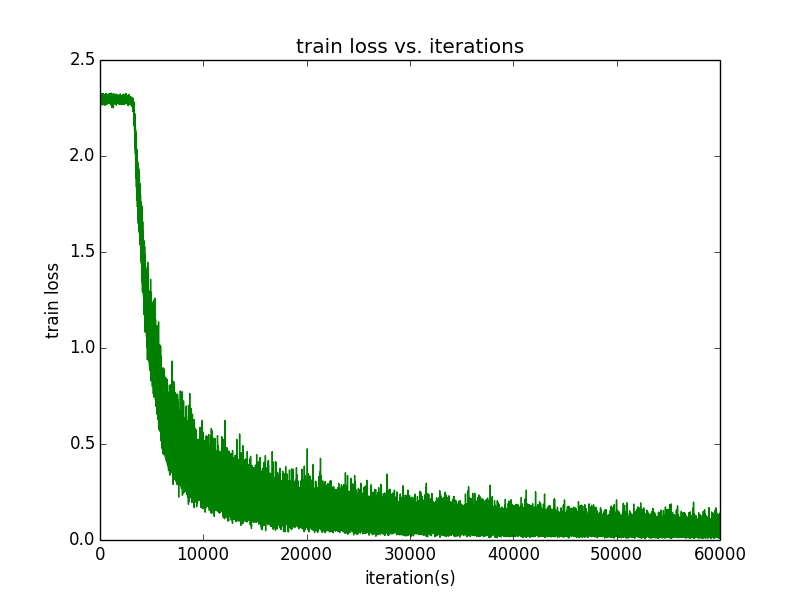
\includegraphics[width=\textwidth]{trainloss2ss}
	\end{minipage}
	\begin{minipage}[t]{0.45\textwidth}
		\centering
		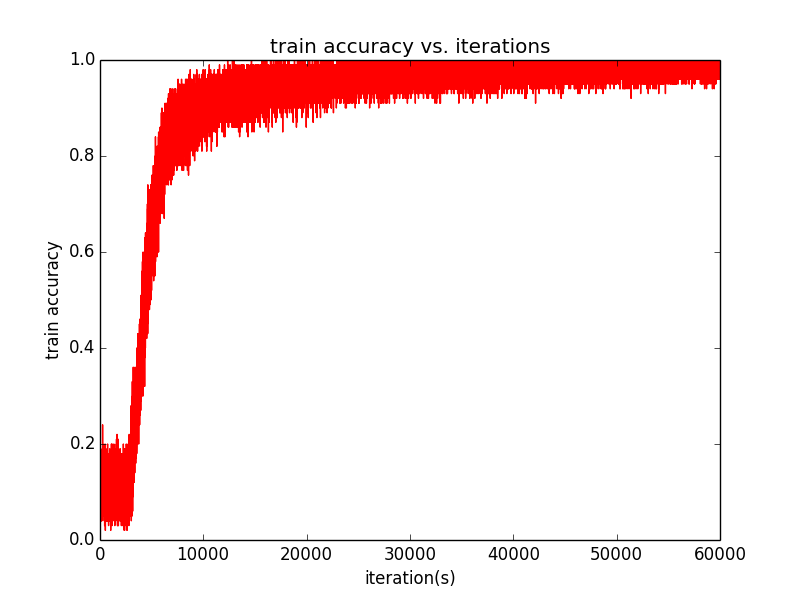
\includegraphics[width=\textwidth]{trainacc2ss}
	\end{minipage}
	\caption{\label{traincurve24}train loss curve and train accuracy curve with two hidden layers, Sigmoid activation function and SoftmaxCrossEntropyLoss}
\end{figure}
\begin{figure}[!ht]
	\centering
	\begin{minipage}[t]{0.45\textwidth}
		\centering
		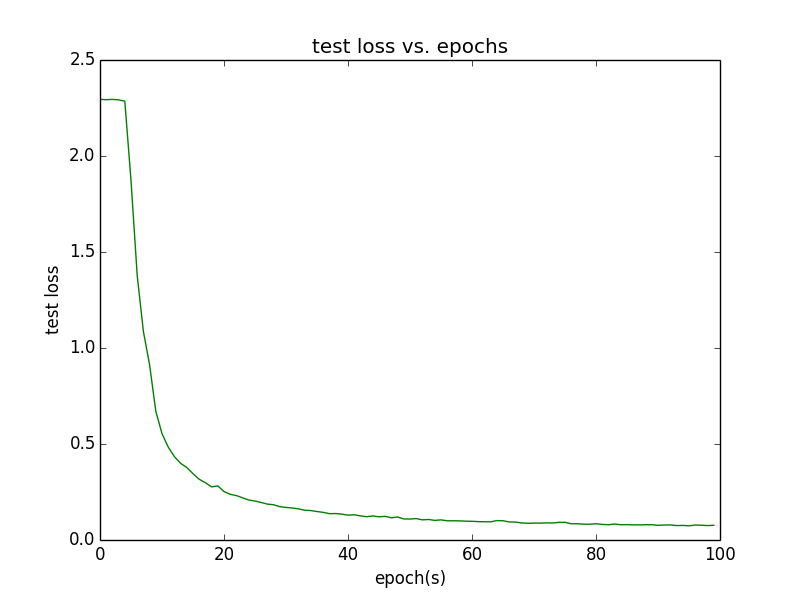
\includegraphics[width=\textwidth]{testloss2ss}
	\end{minipage}
	\begin{minipage}[t]{0.45\textwidth}
		\centering
		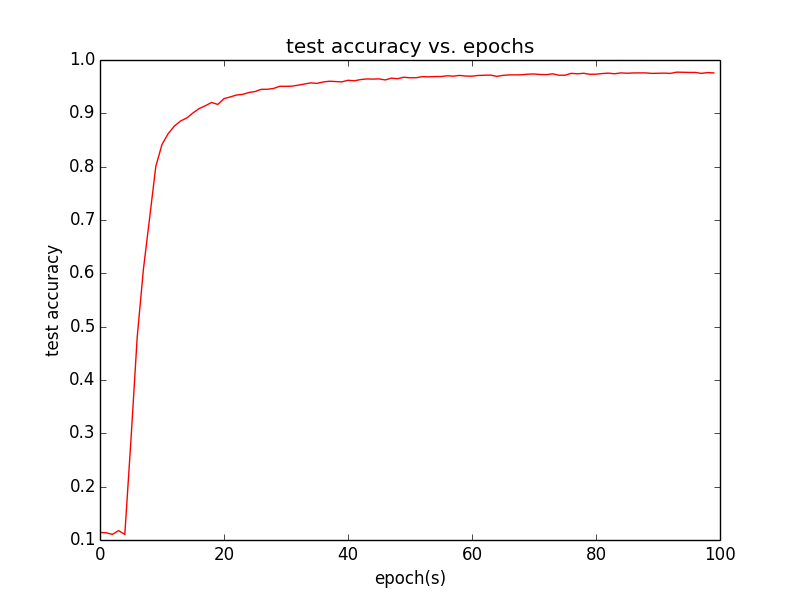
\includegraphics[width=\textwidth]{testacc2ss}
	\end{minipage}
	\caption{\label{testcurve24}test loss curve and test accuracy curve with two hidden layers, Sigmoid activation function and SoftmaxCrossEntropyLoss}
\end{figure}

\section{Results}
We summarize all test accuracys and test losses of every experiments as shown in Table \ref{tab3}(In this table, RE represents the experiments using Relu activation function and EuclideanLoss, SE represents the experiments using Sigmoid activation function and EuclideanLoss, RS represents the experiments using Relu activation function and SoftmaxCrossEntropyLoss, SS represents the experiments using Sigmoid activation function and SoftmaxCrossEntropyLoss). From the results, we can find the best chance is the experiments that use Relu activation function and EuclideanLoss with two hidden layers, the test accuracy is $0.983$.

\begin{table}[!ht]
	\centering
	\caption{\label{tab3}Results Summary}
	\begin{tabular}{|c|c|c|c|c|}
		\hline
		Cases & RE & SE & RS & SS \\
		\hline
		Test Acc with one hidden layer & 0.975 & 0.951 & 0.982 & 0.975 \\
		\hline
		Test Loss with one hidden layer & 0.039 & 0.062 & 0.062 & 0.083 \\
		\hline
		Test Acc with two hidden layers & {\color{red} 0.983} & 0.947 & 0.981 & 0.976 \\
		\hline
		Test Loss with two hidden layers & {\color{green} 0.021} & 0.053 & 0.065 & 0.075 \\
		\hline
	\end{tabular}
\end{table}

\subsection{Comparation of Relu and Sigmoid}
From the results we can find that if we use Relu as activation function, we have bigger test accuracy and faster convergence speed. And Sigmoid may result in Gradient disappear, thus for the mnist digits classification, Relu is much better. 

\subsection{Comparation of One hidden layer and Two hidden layers}
From the results we can find that two hidden layers have bigger test accuracy than one hidden layer. But Two hidden layers have more arguments than one hidden layer, thus the training time is much longer and may lead to overfitting.

\subsection{Comparation of EuclideanLoss and SoftmaxCrossEntropyLoss}
From the results we can find SoftmaxCrossEntropyLoss is more smooth than EuclideanLoss and the test accuracy of the two loss functions is close.
\end{document}